\documentclass[11pt]{scrartcl}
\usepackage[utf8]{inputenc}
\usepackage{enumitem}
\usepackage{amsfonts}
\usepackage{bbm}
\usepackage{newtxmath}
%\usepackage[square]{natbib}
\usepackage{amsmath}
\usepackage{mathrsfs,bm}
\usepackage{graphicx,epstopdf,caption}
\usepackage{float,subcaption,setspace,booktabs,multirow,supertabular,lscape,threeparttable}
\usepackage{float,colortbl}
\usepackage{placeins}
\usepackage{indentfirst}
\usepackage{enumitem}
\setlength{\parindent}{0pt} %% noindent for the entire file % or add indent {2em}
\usepackage{geometry}
\geometry{left=0.8in,right=0.8in,top=1in,bottom=0.5in}
\usepackage[noblocks]{authblk}
\usepackage{lipsum}%% a garbage package you don't need except to create examples.
\usepackage{fancyhdr}
\usepackage[svgnames]{xcolor}
\usepackage{listings}
\usepackage{verbatim}
\usepackage[round, semicolon, sort]{natbib}
\setlength{\parindent}{2em}
\setlength{\belowcaptionskip}{-10pt}
\usepackage[font={footnotesize, it}]{caption}

\pagestyle{fancy}
\lhead{CSCI 5561}  % set your name here
\chead{\large\textbf{Homework 5 - Stereo Reconstruction}}
\rhead{He Zhou (zhou1354@)}
\renewcommand{\headrulewidth}{0.4pt}

\lstset{language=R,
	basicstyle=\small\ttfamily,
	stringstyle=\color{DarkGreen},
	otherkeywords={0,1,2,3,4,5,6,7,8,9},
	morekeywords={TRUE,FALSE},
	deletekeywords={data,frame,length,as,character},
	keywordstyle=\color{blue},
	commentstyle=\color{DarkGreen},
}
\usepackage{Sweave}
\graphicspath{{Figures/}}  % set the path of figures
\usepackage{blindtext}
\usepackage{scrextend}
\addtokomafont{labelinglabel}{\bfseries}
\usepackage{appendix}
\usepackage[linesnumbered,ruled,vlined]{algorithm2e}

\usepackage{algpseudocode}  
\usepackage{hyperref}
\hypersetup{
    colorlinks=true,
    linkcolor=blue,
    filecolor=blue,      
    urlcolor=blue,
    citecolor=cyan,
}

\newcommand{\cX}{\mathcal{X}}
\newcommand{\cR}{\mathcal{R}}
\newcommand{\cV}{\mathcal{V}}
\newcommand{\bw}{\mathbf{w}}

	

\begin{document}

\title{CSCI 5561}
\author{\Large Homework 5 -- Stereo Reconstruction\\
	He Zhou}  %% set your name on the main page
%\date{\vspace{-5ex}}  % suppress the output of date
\maketitle
\newpage

The goal of this assignment is to implement a stereo reconstruction algorithm on two given view images, $\mathcal{I}_1$ and $\mathcal{I}_2$, shown in \autoref{fig:two-images}.
\begin{figure}[ht!]
	\begin{center}
		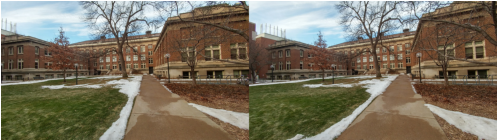
\includegraphics[width=0.7\linewidth]{two_images.png}
	\end{center}
	\caption{Two view images $\mathcal{I}_1$ and $\mathcal{I}_2$.}
	\label{fig:two-images}
\end{figure}
\paragraph{SIFT Feature Matching:}
Function \texttt{find\_match()} uses \texttt{OpenCV} SIFT to extract keypoints and match between two views based on  k-nearest neighbor search. The matches are filtered using the ratio test with threshold $0.7$ and bidirectional consistency check. This function is the same as that in Homework 2. The matched points between images $\mathcal{I}_1$ and $\mathcal{I}_2$ are shown in \autoref{fig:SIFT-match}.

\begin{figure}[ht!]
	\begin{center}
		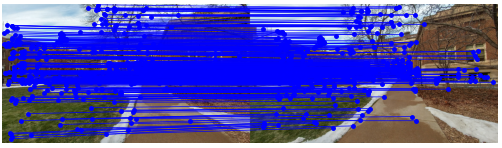
\includegraphics[width=0.8\linewidth]{SIFT_match.png}
	\end{center}
	\caption{Match points between $\mathcal{I}_1$ and $\mathcal{I}_2$ using SIFT features.}
	\label{fig:SIFT-match}
\end{figure}

\paragraph{Fundamental Matrix Computation:} 
Function \texttt{compute\_F()} computes a fundamental matrix by the 8-point algorithm within RANSAC. When implementing RANSAC, the threshold is set to be $0.01$ and the number of iteration is set to be $1000$. SVD clean-up is used to make the rank of the fundamental matrix to be 2. The validity of the fundamental matrix is verified by visualizing epipolar lines as shown in \autoref{fig:epipolar_lines}. 

\begin{figure}[ht!]
	\begin{center}
		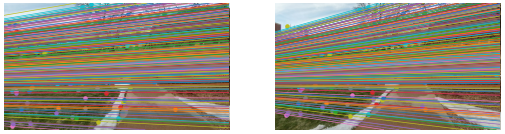
\includegraphics[width=0.8\linewidth]{epipolar_lines.png}
	\end{center}
	\caption{The epipolar lines based on the fundamental matrix.}
	\label{fig:epipolar_lines}
\end{figure}

\paragraph{Triangulation and Pose Disambiguation:}
Function \texttt{triangulation()} uses linear triangulation method to reconstruct 3D points given camera pose and correspondences. Then given four configurations of relative  camera pose and reconstructed points, function \texttt{disambiguate\_pose()} finds the best camera pose by verifying through 3D point triangulation. We find the 3D points that are in front of both cameras by checking the Cheirality condition. Four configurations produce 93, 11, 309 and 391 valid points respectively and the fourth one gives the maximum number of valid points (391), and therefore is the best configuration. The camera pose configurations with point cloud are shown in \autoref{fig:camera}.

\begin{figure}[ht!]
\centering
\begin{subfigure}{.5\textwidth}
	\centering
	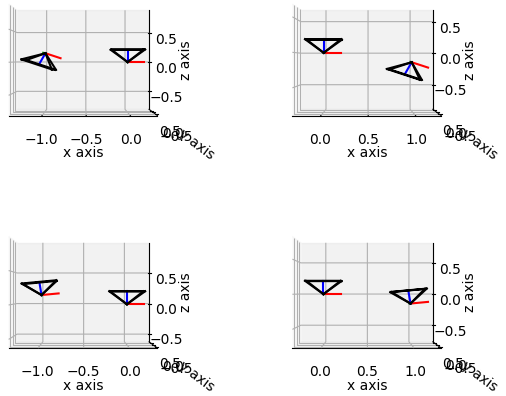
\includegraphics[width=.75\linewidth]{camera_poses.png}
\end{subfigure}%
\begin{subfigure}{.5\textwidth}
	\centering
	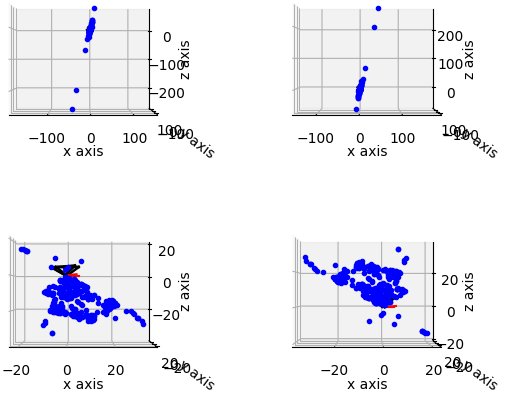
\includegraphics[width=.75\linewidth]{triangulation_93_309_11_391.png}
\end{subfigure}
\caption{Four camera pose configurations with point cloud. The number of validation points are 93, 11, 309, and 391 respectively.}
\label{fig:camera}
\end{figure}

\paragraph{Stereo Rectification and Match:}
Given the disambiguated camera pose, function \texttt{compute\_rectification()} find the rectification rotation matrix $R_\text{rect}$ and computes the rectification homographies $H_1=KR_\text{rect} K^{-1}$ and $H_2=KR_\text{rect} R^\transp K^{-1}$. The rectified images $\tilde{\mathcal{I}}_1$ and $\tilde{\mathcal{I}}_2$ are shown in \autoref{fig:stereo_rectification}. This rectification sends the epipoles to infinity and makes the epipolar line to be the horizontal line.

\begin{figure}[ht!]
	\begin{center}
		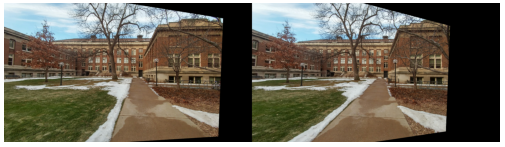
\includegraphics[width=0.8\linewidth]{stereo_rectification.png}
	\end{center}
	\caption{The rectified images $\tilde{\mathcal{I}}_1$ and $\tilde{\mathcal{I}}_2$.}
	\label{fig:stereo_rectification}
\end{figure}

To visualize the stereo match, function \texttt{dense\_match()} computes the dense matches across all pixels, i.e., the disparity matrix. Given a pixel, $\mathbf{u}$, we  sweep along its epipolar line (which is the horizontal line after rectification) and find the disparity $d$ that produces the best match, i.e.,
\begin{equation*}
	d=\arg\min_{i}\left\{
	d_{\mathbf{u}}^1 - d_{\mathbf{u}-(i,0)}^2: i=0,1,\cdots,u_x-1
	\right\},
\end{equation*}
where $d_{\mathbf{u}}^1$ is the dense SIFT descriptor at $\mathbf{u}$ on image $\tilde{\mathcal{I}}_1$ and $d_{\mathbf{u}-(i,0)}^2$ is the SIFT descriptor at $\mathbf{u}-(i,0)$ on image $\tilde{\mathcal{I}}_2$ and $u_x$ is the x-coordinate of pixel $\mathbf{u}$. For pixels out of the range of the image $\tilde{\mathcal{I}}_1$, we simply set the disparity as $d=0$. The visualization of the stereo match is shown in \autoref{fig:stereo_match}.

\begin{figure}[ht!]
	\begin{center}
		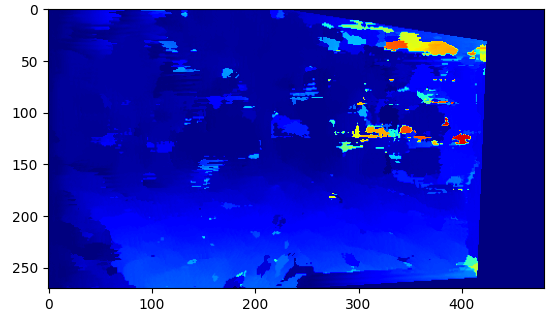
\includegraphics[width=0.6\linewidth]{stereo_match.png}
	\end{center}
	\caption{Visualization of stereo match.}
	\label{fig:stereo_match}
\end{figure}















\nocite*{}  
%\bibliographystyle{apalike}  %disordered
%\bibliographystyle{plain}  %ordered by auther
%\bibliographystyle{unsrt}  %ordered as referenced
\bibliographystyle{IEEEtranN}
\bibliography{bibfile}






\end{document}